\documentclass[11pt]{article}
%%%%%%%%%%%%%%%%%%%%%%%%%%%%%%%% Algunos Paquetes Necesarios 
\usepackage{fancyhdr, graphicx, wrapfig,lipsum}
\usepackage[latin1]{inputenc}% Language
\usepackage{pgf,tikz,pgfplots}
\usepackage{xcolor}
\usepackage{mathrsfs}
\usepackage{fancybox}
\usepackage{subcaption}
\usetikzlibrary{arrows}
\pagestyle{empty}
\usepackage[margin=1in]{geometry} % Margins														
\usepackage{amssymb}
\usepackage{multicol}
\usepackage{amsmath, amsthm, amsfonts}
\usepackage{longtable} % Table accross multiple pages
\usepackage{hyperref}  % Use Hyperlinks
\usepackage{enumitem} % Reduce space in enumerate
\usepackage{txfonts}
\usepackage{float}
\usepackage{wrapfig}
\usepackage{lipsum}
\usepackage[pangram]{blindtext}
\usepackage{vmargin}


\setpapersize{A4}
\setmargins
{3cm}       % margen izquierdo
{1cm}                        % margen superior
{15.5cm}                      % anchura del texto
{24cm}                    % altura del texto
{10pt}                           % altura de los encabezados
{0.7cm}                           % espacio entre el texto y los encabezados
{0pt}                             % altura del pie de página
{1cm}       
\newcommand{\RName}{Rub\'i Esmeralda Ram\'irez Mili\'an}
\newcommand{\JName}{Jorge Alejandro Rodr\'iguez Aldana}
\newcommand{\AName}{Jorge Alejandro \'Avalos Haidacher}
\newcommand{\myDate}{Diciembre de 2019}
\newcommand{\RCarnet}{201804565}
\newcommand{\JCarnet}{201804}
\newcommand{\ACarnet}{201805}
\newcommand{\myCourse}{An\'alisis de variable Compleja 1}
\newcommand{\degre}{\ensuremath{^\circ}}

\newcommand{\R}{\mathbb{R}}
\newcommand{\F}{\mathbf{F}}
\newcommand{\vi}{\mathbf{\hat{i}}}
\newcommand{\vj}{\mathbf{\hat{j}}}
\newcommand{\vk}{\mathbf{\hat{k}}}
\def\proof{\paragraph{Demostraci\'on: \\}}
\def\endproof{\hfill$\blacksquare$}

\def\exercise{\paragraph{Soluci\'on:\\}}
\def\endexercise{\hfill$\square$}

%%%%%%%%%%%%%%%%%%%%%%%%%%%%%%%%%%% Tema - BEGIN
\newtheoremstyle{Tema}% name of the style to be used
  {4mm}% measure of space to leave above the theorem. E.g.: 3pt
  {2mm}% measure of space to leave below the theorem. E.g.: 3pt
  {}% name of font to use in the body of the theorem
  {}% measure of space to indent
  {\bfseries}% name of head font
  {\newline}% punctuation between head and body
  {20mm}% space after theorem head
  {45mm}% Manually specify head

\theoremstyle{Tema} \newtheorem{Tema}{Tema} %%%%% Template para Temas
\theoremstyle{Tema} \newtheorem{serie}{Serie}              %%%%%  Template para Series de ejercicios
\theoremstyle{Tema} \newtheorem{ejercicio}{Ejercicio}    %%%%%  Template para Ejercicios
%%%%%%%%%%%%%%%%%%%%%%%%%%%%%%%%%%% Tema - END


%%%%%%%%%%%%%%%%%%%%%%%%%%%%%%%%%%% Encabezado - BEGIN %%%%%%%%%%
\fancypagestyle{firststyle}
{
\renewcommand{\headrulewidth}{0.5pt}
\fancyhead[L]{
			\textbf{Universidad de San Carlos de Guatemala} \\
			\textbf{Escuela de Ciencias F\'isicas y Matem\'aticas}\\
			  %%%%%%%%%% Agregar nombre del curso 
			\textbf{\RName-\RCarnet} \\ 
			\textbf{\JName-\JCarnet} \\
			\textbf{\AName- \ACarnet} \\
			 %%%%%%%%%%%%%%%%%%%%%% Agregar fecha en formato: Enero 15, 2015
			}
\fancyhead[R]{}
}
%%%%%%%%%%%%%%%%%%%%%%%%%%%%%%%%%%% Encabezado - END %%%%%%%%%%

%%%%%%%%%%%%%%%%%%%%%%%%%%%%%%%%%%% Encabezado (pagina 2 en adelante) - BEGIN %%%
\fancypagestyle{allStyle}
{
\renewcommand{\headrulewidth}{0.8pt}
\fancyhead[R]{
			\emph{Tarea 1 $-$ \myCourse} %%%% Modificar n\'umero de examen parcial y nombre del curso
			}
\fancyhead[L]{}  
\fancyfoot[C]{}
\fancyfoot[R]{\thepage}
}
%%%%%%%%%%%%%%%%%%%%%%%%%%%%%%%%%%% Encabezado (pagina 2 en adelante) - END %%%

\date{}
\setlength{\headheight}{0.9in} % fixes \headheight warning

\begin{document} %%%%%%%%%%%%%%%%%%%%%%%% BEGIN%%%%%%%%%%%%%%

\pagestyle{allStyle}

\thispagestyle{firststyle}
%%%%%%%%%%%%%%%%%%%%%%%%%%%%%%%%% Titulo - BEGIN
\begin{center}
\LARGE
 \text{Tarea 1}\\\normalsize \myCourse % Modificar el N\'umero del examen parcial
\medskip
\hrule height 1.5pt
\end{center}

	\section*{\textbf{Problema 1.} }
\bigskip




\section*{\textbf{Problema 2.} }


\begin{proof}
\begin{equation*}
\left|\dfrac{\alpha+z}{1+\overline{\alpha}z}\right|\leq 1
\end{equation*}

\begin{equation*}
\Leftrightarrow \left|{\alpha+z}\right|\leq \left|{1+\overline{\alpha}z}\right|
\end{equation*}

\begin{equation*}
\Leftrightarrow \left|{\alpha+z}\right|^2\leq \left|{1+\overline{\alpha}z}\right|^2
\end{equation*}

\begin{equation*}
\Leftrightarrow ({\alpha+z})(\overline{\alpha+z})\leq ({1+\overline{\alpha}z})\overline{({1+\overline{\alpha}z})}
\end{equation*}


\begin{equation*}
\Leftrightarrow ({\alpha+z})(\overline{z}+\overline{\alpha})\leq ({1+\overline{\alpha}z})({1+\overline{z}\alpha})
\end{equation*}


\begin{equation*}
\Leftrightarrow \alpha \overline{z}+ \alpha\overline{\alpha}+z\overline{z}+z\overline{a}\leq {1+\overline{\alpha}z +\overline{z}\alpha+z\overline{z}\alpha\overline{\alpha}}
\end{equation*}

\begin{equation*}
\Leftrightarrow \alpha\overline{\alpha}+z\overline{z}\leq {1 +z\overline{z}\alpha\overline{\alpha}}
\end{equation*}

\begin{equation*}
\Leftrightarrow |\alpha|^2+|z|^2\leq {1+|z|^2 |\alpha |^2}
\end{equation*}

\begin{equation*}
\Leftrightarrow |\alpha|^2- 1-|z|^2 |\alpha |^2+|z|^2\leq 0
\end{equation*}


\begin{equation*}
\Leftrightarrow |\alpha|^2- 1-|z|^2 (|\alpha |^2-1)\leq 0
\end{equation*}


\begin{equation}
\Leftrightarrow(1-|z|^2 ) (|\alpha |^2-1)\leq 0
\end{equation}

Como $|z|\leq 1$, $ \Rightarrow |z|^2\leq 1 $, $0\leq 1-|z|^2$. Adem\'as $ |\alpha|<1 $, $ \Rightarrow |\alpha|^2\leq 1 $, $ |\alpha|^2-1<0$.  Entonces (1) si se cumple.   

\end{proof}


La igualdad se alcanza cuando el $|z|=1$





\section*{\textbf{Problema 3.} }

\begin{exercise}

Para resolverlo, se usa congruencias (n$ \in  \mathbb{Z}$ )
\begin{center}
\begin{tabular}{|c|c|}
		\hline
			$ n\equiv 0 $ $mod$ 8&$ n^2\equiv 0^2\equiv 0$ $ mod $ 8\\
		\hline
	$ n\equiv 1 $ $mod $ 8&$ n^2\equiv 1^2\equiv 1$ $ mod $ 8\\
	\hline
	$ n\equiv 2 $ $mod $ 8&$ n^2\equiv 2^2\equiv 4 $ $ mod $ 8\\
	\hline
	$ n\equiv 3 $ $mod $ 8&$ n^2\equiv 3^2\equiv 1$ $ mod $ 8\\
	\hline
	$ n\equiv 4 $ $mod$ 8&$ n^2\equiv 4^2\equiv 0$ $ mod $ 8\\
	\hline
	$ n\equiv 5 $ $mod $ 8&$ n^2\equiv 5^2\equiv 1$ $ mod $ 8\\
	\hline
	$ n\equiv 6 $ $mod $ 8&$ n^2\equiv 6^2\equiv 4 $ $ mod $ 8\\
	\hline
	$ n\equiv 7 $ $mod $ 8&$ n^2\equiv 7^2\equiv 1$ $ mod $ 8\\
	\hline


\end{tabular}
\end{center}

Ahora por De Moivre:

$ arg({z^{(8n+1)}}^2)= (8n+1)^2\frac{\pi}{4}= (8k_1+1)\frac{\pi}{4} =arg(z)$

De modo semejante:
\medskip

$ arg({z^{(8n+2)}}^2)=(8n+2)^2\frac{\pi}{4}= (8k_2+4)\frac{\pi}{4}= arg(-z^0)$

$ arg({z^{(8n+3)}}^2)=(8n+3)^2\frac{\pi}{4}= (8k_3+1)\frac{\pi}{4}=arg(z)$


$ arg({z^{(8n+4)}}^2)=(8n+4)^2\frac{\pi}{4}= (8k_4)\frac{\pi}{4}=arg(z^0)$

$ arg({z^{(8n+5)}}^2)=(8n+5)^2\frac{\pi}{4}= (8k_5+1)\frac{\pi}{4}= arg(z)$

$ arg({z^{(8n+6)}}^2)=(8n+6)^2\frac{\pi}{4}= (8k_6+4)\frac{\pi}{4}=arg(-z^0)$


$ arg({z^{(8n+7)}}^2)=(8n+7)^2\frac{\pi}{4}= (8k_7+1)\frac{\pi}{4}=arg(z)$

$ arg({z^{(8n)}}^2)=(8n)^2\frac{\pi}{4}= (8k_8)\frac{\pi}{4}=arg(z^0)$


\bigskip

Y como $ |z|=1 $:

\begin{equation*}
\left({z^1}^2+{z^2}^2+{z^3}^2+{z^4}^2+\cdots{z^{12}}^2\right)=6z=6e^{i\frac{\pi}{4}}
\end{equation*}


\begin{equation*}
\left(\dfrac{1}{{z^1}^2}+\dfrac{1}{{z^2}^2}+\dfrac{1}{{z^3}^2}+\dfrac{1}{{z^4}^2}+\cdots\dfrac{1}{{z^{12}}^2}\right)=6\overline{z}=6e^{-i\frac{\pi}{4}}
\end{equation*}

Por tanto:

\begin{equation*}
\left({z^1}^2+{z^2}^2+{z^3}^2+{z^4}^2+\cdots{z^{12}}^2\right)\left(\dfrac{1}{{z^1}^2}+\dfrac{1}{{z^2}^2}+\dfrac{1}{{z^3}^2}+\dfrac{1}{{z^4}^2}+\cdots\dfrac{1}{{z^{12}}^2}\right)=36
\end{equation*}
\end{exercise}

\section*{\textbf{Problema 4.} }




\section*{\textbf{Problema 5.} }



\begin{figure}[H]
	\centering
	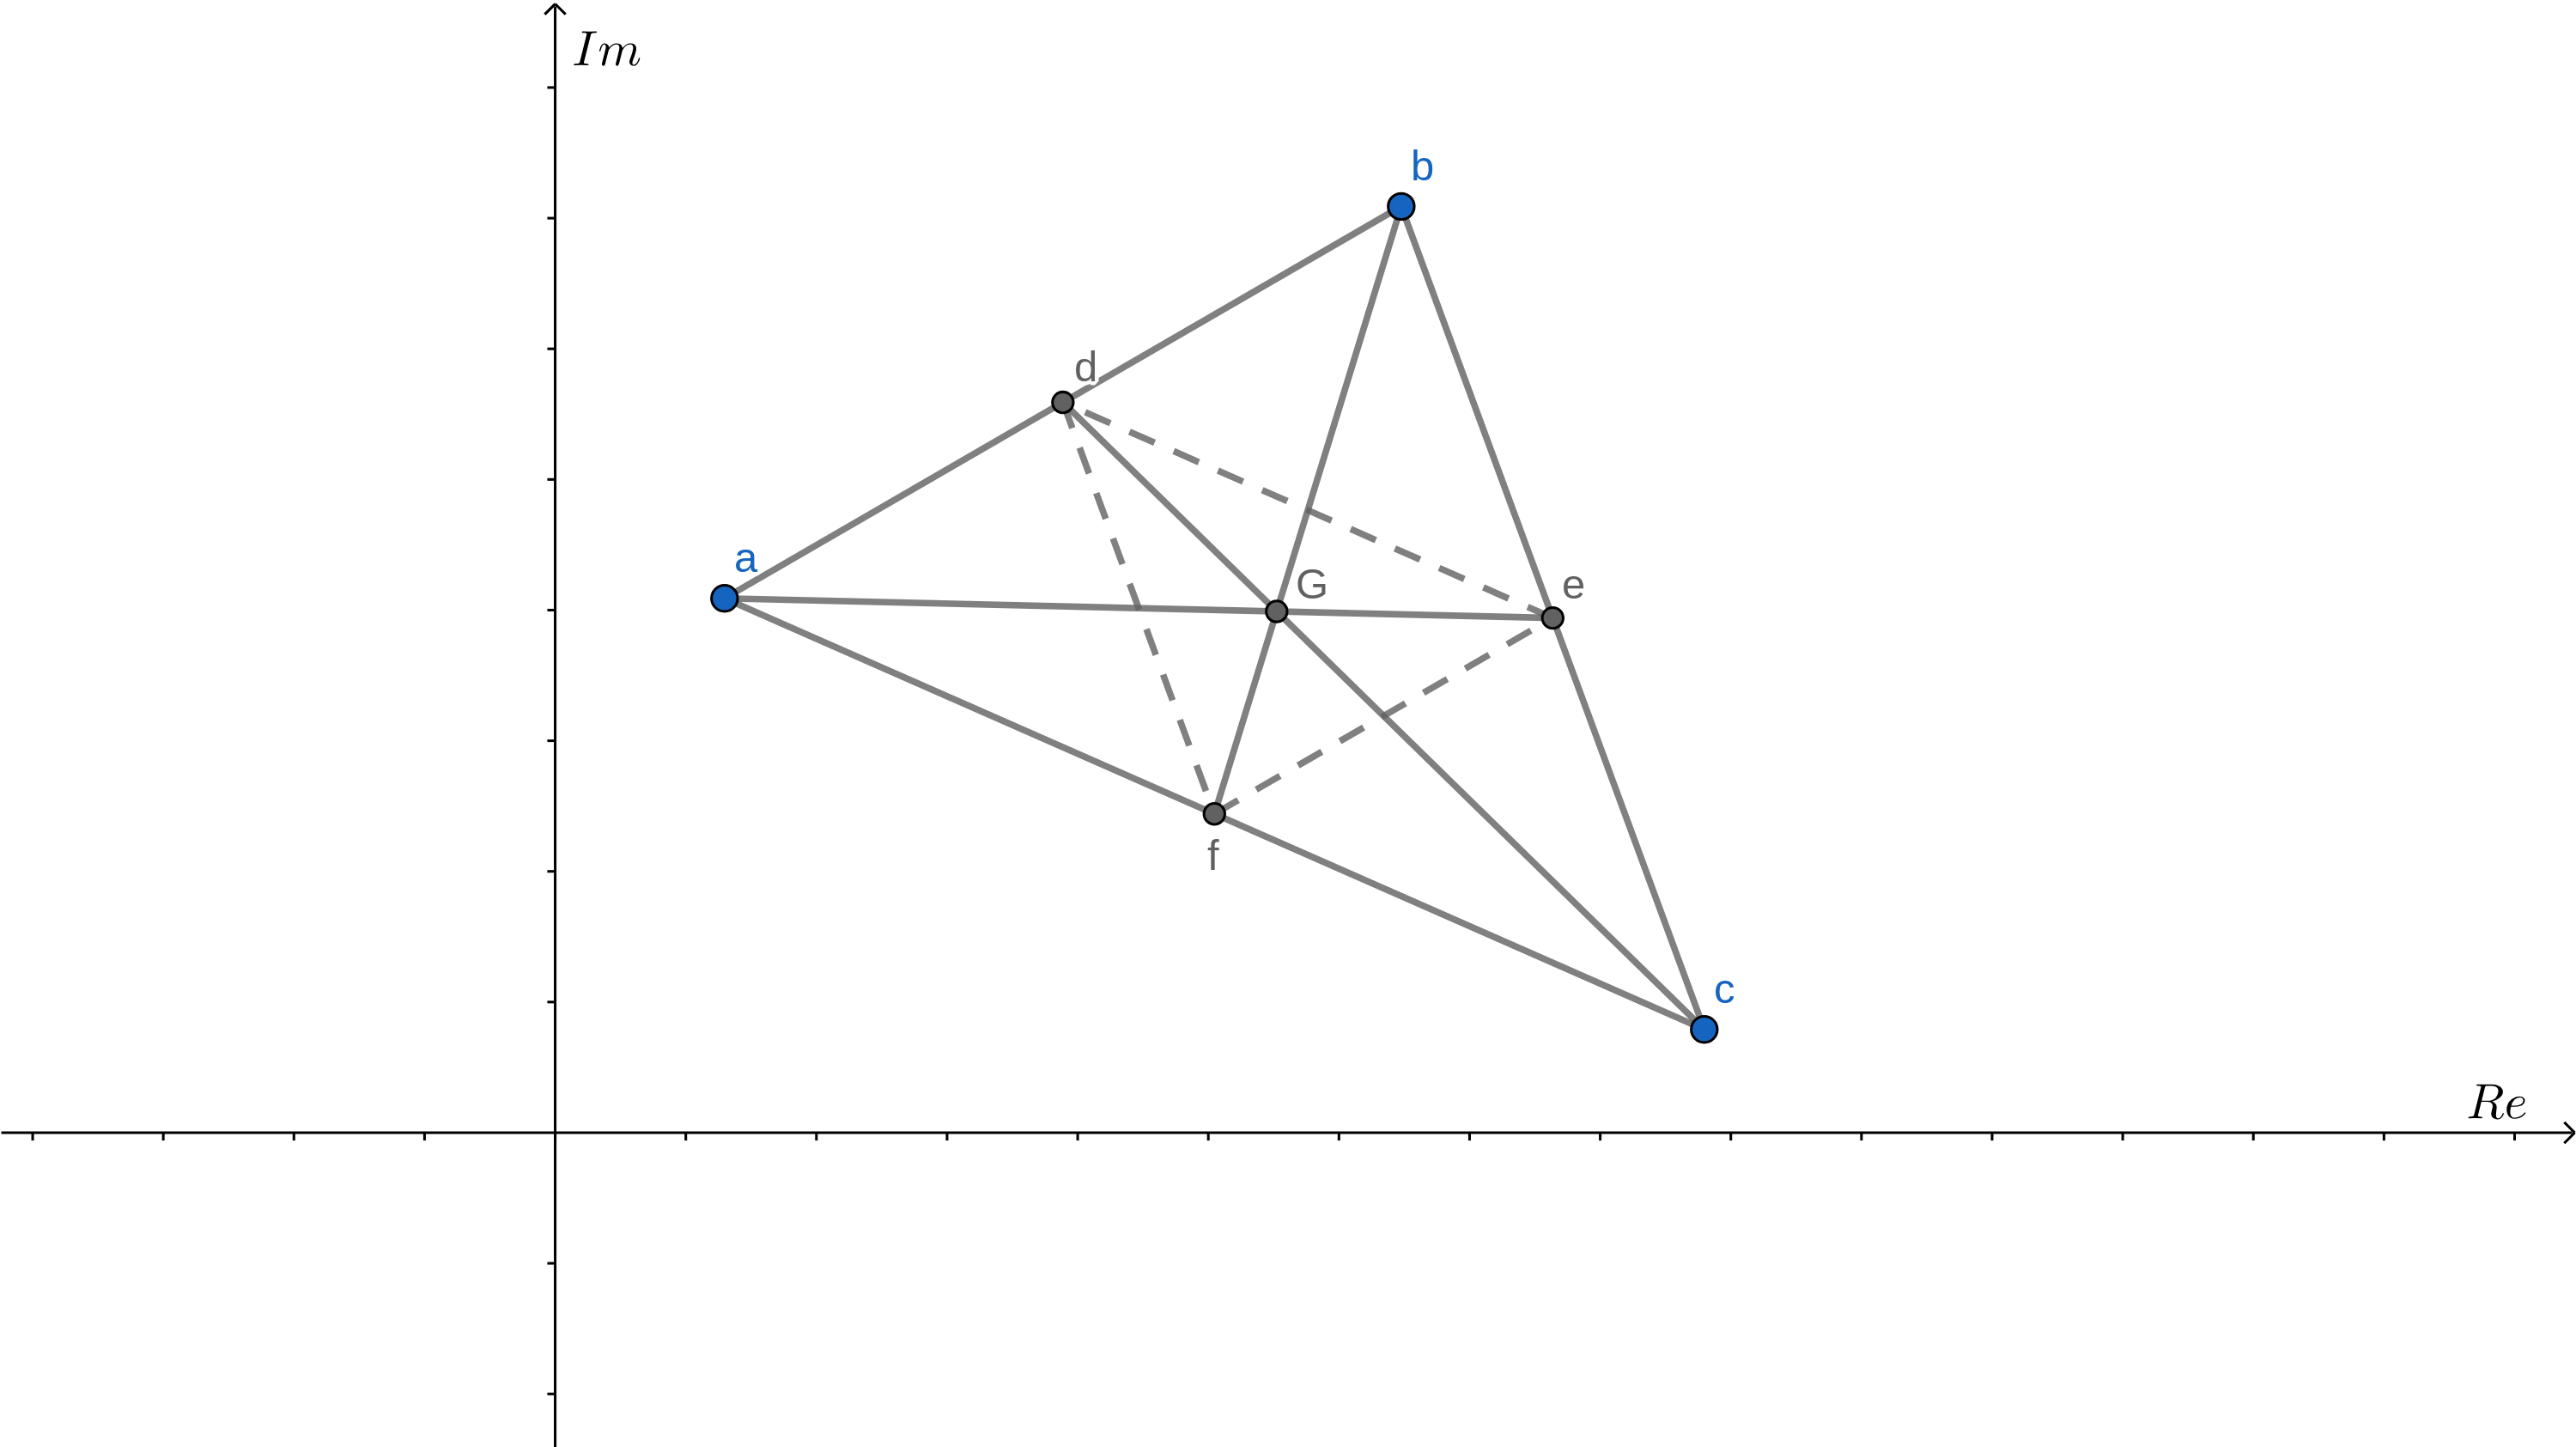
\includegraphics[width=0.7\linewidth]{5}
\end{figure}
\begin{proof}
	


Sean $ a,b,c  \in \mathbb{C}$, entonces son de la forma:
\begin{center}
\begin{tabular}{c}
	$ a= \alpha_1+i\beta_1 $\\  
	$ b= \alpha_2+i\beta_2 $\\ 
	$ c= \alpha_3+i\beta_3 $\\ 
\end{tabular} 	
\end{center}

Sean $ d, e, f $ los puntos medios de los lados $ \vec{ba} $, $ \vec{cb} $, $ \vec{ca} $. Entonces:

\begin{center}
	\begin{equation}
	\begin{tabular}{c}
		$ d=\gamma_1+i\omega_1= \dfrac{a+b}{2} $\\
		\\  
		$ e= \gamma_2+i\omega_2=\dfrac{c+b}{2} $\\ 
		\\
		$ f=\gamma_3+i\omega_3= \dfrac{a+c}{2}$\\ 
	\end{tabular} 	
	\end{equation}
\end{center}

Por lo que $  \vec{cd} , \vec{ae},\vec{bf}$ son las medianas de los lados $ \vec{ba} $, $ \vec{cb} $, $ \vec{ca} $ respectivamente y G es el centroide por lo que: $|bG|=2|fG|, |aG|=2|eG|, |cG|=2|dG|   $. Por lo que $ G=x +iy $ se puede escribir en funci\'on de los puntos $ a,b,c,d,e,f$


$ |bG|=2|fG| $


\begin{center}
\begin{equation*}
\begin{tabular}{lr}
$2(x-\gamma_1)=\alpha_2-x $& $2(x-\omega_1)=\beta_2-y$\\
$ x=\dfrac{\alpha_2-2\gamma_1}{3} $&  $y=\dfrac{\beta_2-2\omega_1}{3}$\\
\end{tabular} 
\end{equation*}
\end{center}

Por lo que $ G=\dfrac{\alpha_2-2\gamma_1}{3}+ \dfrac{\beta_2-2\omega_1}{3}i= \dfrac{b+2f}{3} $. Y an\'alogamente se puede obtener $ G= \dfrac{c+2d}{3}=\dfrac{a+2e}{3}$


Luego por estas igualdades se tiene que:

\begin{center}
	\begin{equation*}
	\begin{tabular}{lc}
	& $G=\dfrac{a+2e}{3} $\\
	\\  
	 &$G=\dfrac{c+2d}{3} $\\ 
	 \\
	 +&$G=\dfrac{b+2f}{3}$\\
	\hline 
	\\
	 &$3G=\dfrac{a+b+c+2(e+d+f)}{3}$\\
	\end{tabular} 	
	\end{equation*}
	\end{center}

Luego sumando las tres ecuaciones de (2):
$ d+e+f=\dfrac{2a+2b+2c}{2}=a+b+c $. Y sustituyendo en la ecuaci\'on obtenida anteriormente:

\begin{equation*}
3G=\dfrac{a+b+c+2(a+b+c)}{3}=\dfrac{3(a+b+c)}{3}=a+b+c
\end{equation*}


\begin{equation*}
G=\dfrac{a+b+c}{3}
\end{equation*}
\end{proof}
\section*{\textbf{Problema 6.} }

\begin{proof}
Se tiene que:

\begin{equation*}
\dfrac{\sin(2n\theta)}{\sin(\theta)}=\dfrac{Im(e^{2in\theta})}{Im(e^{i\theta})}=\dfrac{\frac{1}{2i}(e^{2in\theta}-e^{-2in\theta})}{\frac{1}{2i}(e^{i\theta}-e^{-i\theta})} = \dfrac{a^{2n}-b^{2n}}{a-b}
\end{equation*}
		
		
	Donde $ a = e^{i\theta}  $	y $ b=e^{-i\theta} $, por lo que:
	
	
	
	\begin{equation*}
	\dfrac{\sin(2n\theta)}{\sin(\theta)}= a^{2n-1}+a^{2n-2}b+\cdots+ab^{2n-2}+b^{2n-1}
	\end{equation*}
		
		
		\begin{equation*}
		= {e^{(i\theta)}}^{2n-1}+{e^{(i\theta)}}^{2n-2}{e^{-i\theta}}+\cdots+{e^{(i\theta)}}^{n}{e^{(-i\theta)}}^{n-1}+{e^{(i\theta)}}^{n-1}{e^{(-i\theta)}}^{n}+\cdots+{e^{i\theta}}{e^{(-i\theta)}}^{2n-2}+{e^{(-i\theta)}}^{2n-1}
		\end{equation*}
		
		
			\begin{equation*}
		= {e^{(i\theta)}}^{2n-1}+{e^{(i\theta)}}^{2n-3}+\cdots+e^{i\theta}+e^{-i\theta}+
		\cdots +{e^{i\theta}}{e^{(-i\theta)}}^{2n-2}+{e^{(-i\theta)}}^{2n-1}
		\end{equation*}
		
		
		
		\begin{equation*}
		= (e^{(2n-1)i\theta}+e^{-(2n-1)i\theta})+\cdots+(e^{i\theta}+e^{-i\theta})
		\end{equation*}
		
		
		
			
		\begin{equation*}
		= 2 (\cos \theta+\cos 3\theta+\cdots+\cos(2n-1)\theta)
		\end{equation*}
		
		\begin{equation*}
		= 2 (\cos \theta+\cos 3\theta+\cdots+\cos(2n-1)\theta)
		\end{equation*}
		
		\begin{equation*}
		\dfrac{\sin(2n\theta)}{2\sin(\theta)}=\cos \theta+\cos 3\theta+\cdots+\cos(2n-1)\theta
		\end{equation*}
		
		
		\end{proof}
		\section*{\textbf{Problema 7.} }

	
		
		\section*{\textbf{Problema 8.} }
		 
		
		\begin{exercise}
		Sea $ z^n =1 $, se tiene que $ z^n-1=0 $
		Este polinomio tiene n ra\'ices de la forma $ \xi_k $ con lo que se puede escribir:
		
		\begin{equation}
		z^n-1=(z-1)(z-\xi)(z-\xi_2)\dots(z-\xi_{n-1})
		\end{equation}
		
		Pero $ \xi_k $ se puede escribir en la forma :
		$ e^{\frac{2\pi i}{n}k}= e^{\left(\frac{2\pi i}{n}\right)^k}$ 
		
		Con lo que se puede obtener la relaci\'on entre las raices:
		 
		 
		 \begin{center}
		 	\begin{equation*}
		 	\begin{tabular}{c}
		 	$ \xi_1= e^{\left(\frac{2\pi i}{n}\right)}$\\  
		 	$ \xi_2= e^{\left(\frac{2\pi i}{n}\right)^2}=\xi_1^2$\\ 
		 	$\vdots$\\		 	
		 	$ \xi_{n-1}= e^{\left(\frac{2\pi i}{n}\right)^{n-1}}=\xi_1^{n-1}$\\ 
		 	\end{tabular} 	
		 	\end{equation*}
		 \end{center}
	 
	Por lo que (3) se vuelve de la forma:
	\begin{equation}
	z^n-1=(z-1)(z-\xi_1)(z-\xi_1^2)\dots(z-\xi_1^{n-1})
	\end{equation} 
	
	Por otro lado:
		\begin{equation}
	z^n-1=(z-1)(1+z+z^2+\dots+z^{n-1})
	\end{equation} 
		 
		 
	De (4) y (5) se obtiene lo siguiente:
	\begin{equation}
	f(z)= (z-\xi_1)(z-\xi_1^2)\dots(z-\xi_1^{n-1})=(1+z+z^2+\dots+z^{n-1})
	\end{equation}	 
	
	Si se valua $f(1)$ en (6) se obtiene la expresi\'on pedida:
	
	\begin{equation*}
	f(1)=(1-\xi_1)(1-\xi_1^2)\dots(1-\xi_1^{n-1})=(1+1+1^2+\dots+1^{n-1})=n
	\end{equation*}
	
	\begin{equation}
	(1-\xi)(1-\xi^2)\dots(1-\xi^{n-1})=n
	\end{equation}
		
		\end{exercise}
		
		\section*{\textbf{Problema 9.} }
	
		\section*{\textbf{Problema 10.} }
	
		
		\section*{\textbf{Problema 11.} }
	
		\begin{proof}
			
		La funci\'on $ e^{-x} \sin(x) $ puede escribirse de la forma:	
			
			\begin{equation*}
			e^{-x}\left(\dfrac{e^{ix}-e^{-ix}}{2i}\right)
			\end{equation*}
			
			
			
			\begin{equation*}
			\dfrac{e^{x(i-1)}-e^{x(-i-1)}}{2i}
			\end{equation*}
			
	Ahora la n-\'esima derivada, de la funci\'on exponenecial es:
	
	\begin{equation}
	\dfrac{d^n}{dx^n}\left(	\dfrac{e^{x(i-1)}-e^{x(-i-1)}}{2i}\right)=\left(\dfrac{(i-1)^ne^{x(i-1)}-(-i-1)^ne^{x(-i-1)}}{2i}\right)
	\end{equation}		
			
			
	Por la f\'ormula de De Moivre:
	\begin{equation*}
	(i-1)^n=\sqrt{2}^n\left(\cos\left(\dfrac{3n\pi}{4}\right)+i\sin\left(\dfrac{3n\pi}{4}\right)\right)
	\end{equation*}	
	
	\begin{equation*}
	(-i-1)^n=\sqrt{2}^n\left(\cos\left(\dfrac{5n\pi}{4}\right)+i\sin\left(\dfrac{5n\pi}{4}\right)\right)=
	\sqrt{2}^n\left(\cos\left(\dfrac{-3n\pi}{4}\right)+i\sin\left(\dfrac{-3n\pi}{4}\right)\right)
	\end{equation*}		
			
			
Ahora (8) se escribe como:
\begin{equation*}
\sqrt{2}^ne^{-x}\left(\dfrac{\left(\cos\left(\dfrac{3n\pi}{4}\right)+i\sin\left(\dfrac{3n\pi}{4}\right)\right)e^{ix}-\left(\cos\left(\dfrac{3n\pi}{4}\right)-i\sin\left(\dfrac{3n\pi}{4}\right)\right)e^{-ix}}{2i}\right)
\end{equation*}			
			
Adem\'as $ e^{ix}=\cos x+i\sin x $, 	$ e^{-ix}=\cos x-i\sin x $		
			
Luego la expresi\'on anterior queda como			
	\begin{equation*}
	\sqrt{2}^ne^{-x}\left(\dfrac{\left(\cos\left(\dfrac{3n\pi}{4}\right)+i\sin\left(\dfrac{3n\pi}{4}\right)\right)(\cos x+i\sin x)-\left(\cos\left(\dfrac{3n\pi}{4}\right)-i\sin\left(\dfrac{3n\pi}{4}\right)\right)(\cos x-i\sin x)}{2i}\right)
	\end{equation*}		
			
Expandiendo y cancelando t\'erminos:
	\begin{equation*}
	\sqrt{2}^ne^{-x}\left(\dfrac{2i\left(\sin\left(\dfrac{3n\pi}{4}\right)\cos x+\cos\left(\dfrac{3n\pi}{4}\right)sin x\right)}{2i}\right)
	\end{equation*}	
	
		\begin{equation*}
	\sqrt{2}^ne^{-x}\left(\sin\left(\dfrac{3n\pi}{4}+x\right)\right)
		\end{equation*}		
		
		
			
		\end{proof}
	
\section*{\textbf{Problema 12.} }
 

\section*{\textbf{Problema 13.} }


\section*{\textbf{Problema 14.} }

\begin{exercise}
Sea $ z=a+bi $, entonces $ z^2=a^2-b^2-2abi $, $ \overline{z}^2=a^2-b^2-2abi $. Adem\'as $ |z|^2=2 $
por lo que $ a^2+b^2=2 $.

Ahora operando:
\begin{equation*}
|(z^2-1)(z-1)|^2
\end{equation*}

\begin{equation*}
|(z^2-1)^2|(z-1)|^2
\end{equation*}

\begin{equation*}
(z^2-1)(\overline{z}^2-z)(z-1)(\overline{z}-1)
\end{equation*}

\begin{equation*}
((z\overline{z})^2-z^2-\overline{z}^2+1)(z\overline{z}-z-\overline{z}+1)
\end{equation*}

\begin{equation*}
(|z|^4-z^2-\overline{z}^2+1)(|z|^2+2Re(z)+1)
\end{equation*}

Luego se sustituyen ciertos valores:

\begin{equation*}
(4-2a^2+2b^2+1)(2+2a+1)=(4-2a^2+2(2-a^2)+1)(2+2a+1)
\end{equation*}


 y se define $f(a)$ como:


\begin{equation*}
f(a)=(4-2a^2+4-2a^2+1)(2+2a+1)=(9-2a^2)(3+2a)
\end{equation*}


\begin{equation*}
f(a)=4a^3-6a^2-18a+27
\end{equation*}

Para encontrar el m\'aximo de la funci\'on se deriva y  se iguala a cero, los $ a_n $ para los que $ f'(a)=0 $ se valuan en $ f''(a) $.

\begin{equation*}
f'(a)= 12a^2-12a-18
\end{equation*}

Se tiene $ a_1=\dfrac{1-\sqrt{7}}{2}$  $, a_2=\dfrac{1+\sqrt{7}}{2}$


$ f''\left(\frac{-1-\sqrt{7}}{2}\right) =-12\sqrt{7}<0$

Por lo que $ f(a) $ tiene un m\'aximo en $ \dfrac{1-\sqrt7}{2} $

Valuando en $ f(a) $:


\begin{equation*}
f(a)=4\left(\dfrac{1-\sqrt7}{2}\right)^3-6\left(\dfrac{1-\sqrt7}{2}\right)^2-18\left(\dfrac{1-\sqrt7}{2}\right)+27=17+7\sqrt{7}
\end{equation*}

Entonces $ f(a) $ tiene una m\'aximo en $ 17+7\sqrt{7} $. Pero el m\'aximo que se desea conocer es el de la ra\'iz de de $ f(a) $. Por lo que el valor m\'aximo de $  |(z^2-1)(z-1)|=\sqrt{17+7\sqrt{7}}$

\end{exercise}
\section*{\textbf{Problema 15.} }

%%%%%%%%%%%%%%%%%%%%%%%%%%%%%%%%% Instrucciones - BEGIN

\vspace{0.05 in}

\end{document} %%%%%%%%%%%%%%%%%%%%%%%% BEGIN%%%%%%%%%%%%%%